\documentclass{article}
\usepackage[utf8]{inputenc}
\usepackage[T1]{fontenc}
\usepackage{ngerman}
\usepackage{a4wide}
\usepackage{amsmath}
\usepackage{graphicx}

\usepackage{scrpage2}
\pagestyle{scrheadings}

%=========================
%   INFOS
%=========================

\newcommand{\autoren}{Konstantin Kobs (6414943), Mirco Spilker (6427050)}
\newcommand{\titel}{Optimierung für Studierende der Informatik}
\newcommand{\blattnummer}{1}

%=========================

\ihead{\autoren}
\ohead{Aufgabenblatt \blattnummer}
\ofoot{Aufgaben im Fach "`\titel"', Seite \pagemark}

\setheadsepline{1pt}
\setfootsepline{1pt}

%=========================
%   BEGINN DES DOKUMENTS
%=========================
\begin{document}

\section*{Aufgabe 1}
\subsection*{a)}
\subsubsection*{(i)}

Das gegebene LP-Problem sieht folgendermaßen in der Standardform aus:
\begin{align*}
	\text{maximiere } - x_1 + x_2 - x_3 + 2x_4\\
	\text{unter den Nebenbedingungen}\\
	-7x_1 -x_2+x_3 &\leq 2\\
	5x_2-x_3-x_4 &\leq -7\\
	3x_1+x_2-2x_3+x_4 &\leq 3\\
	-3x_1-x_2+2x_3-x_4 &\leq -3\\
	x_1, x_2, x_3, x_4 &\geq 0
\end{align*}

\subsubsection*{(ii)}

Das gegebene LP-Problem sieht folgendermaßen in der Standardform aus:
\begin{align*}
	\text{maximiere } x_1 - x_2' + x_2'' + x_3 + 2x_4\\
	\text{unter den Nebenbedingungen}\\
	7x_1 + x_2' - x_2'' - 4x_3 &\leq -2\\
	-3x_1 + x_2' - x_2'' - 2x_3 + x_4 &\leq 3\\
	x_2' - x_2'' - 2x_3 - 2x_4 &\leq 5\\
	-x_2' + x_2'' + 2x_3 + 2x_4 &\leq -5\\
	x_4 &\leq 7\\
	x_1, x_2', x_2'', x_3, x_4 &\geq 0
\end{align*}

\subsection*{b)}

\begin{figure*}[h]
	\center
	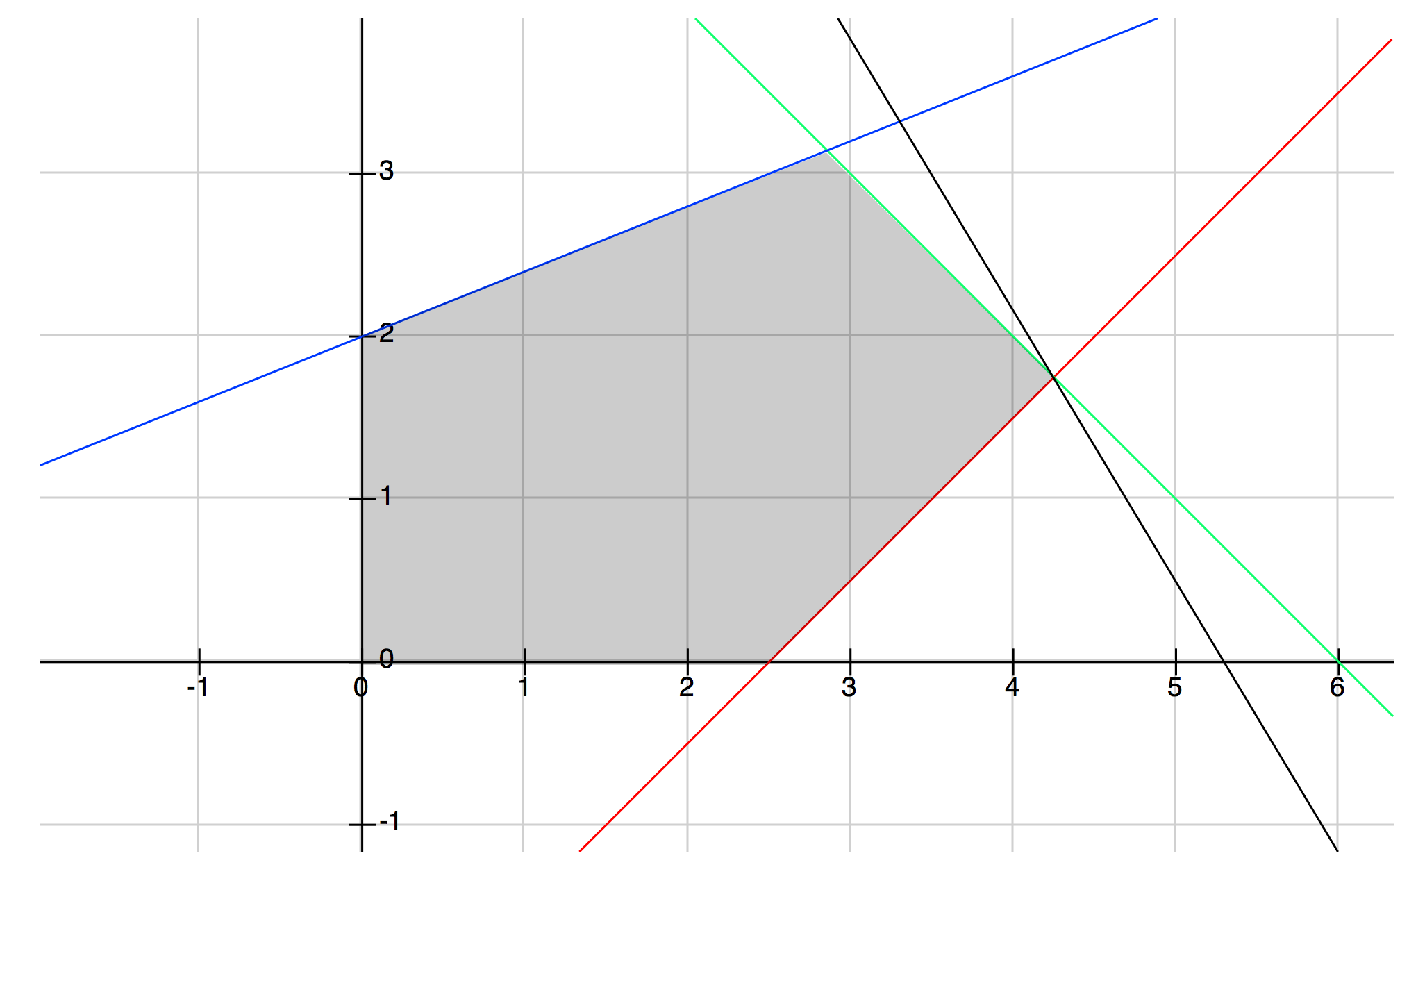
\includegraphics[width=0.5\textwidth]{Graph}
	\caption{Abbildung zu Aufgabe 2b}
	\label{fig:2b}
\end{figure*}

Wir formen die Nebenbedingungen nach $x_2$ um und bekommen:

\begin{align*}
	x_2 &\geq x_1 - \frac{5}{2}\\
	x_2 &\leq 6 - x_1\\
	x_2 &\leq 2 + \frac{2}{5}x_1\\
\end{align*}

Analog erhalten wir für die Zielfunktion $5x_1 + 3x_2 = d$:

$$x_2 = \frac{d}{2} - \frac{5}{3}x_1$$

Eine Visualisierung zeigt das Bild \ref{fig:2b}, wobei die graue Fläche der zulässige Bereich der Zielfunktion ist. Die Funktionen der Nebenbedingungen sind in Rot, Grün und Blau eingezeichnet. Die Zielfunktion in Schwarz. Man kann erkennen, dass die optimale Lösung für das LP-Problem im Schnittpunkt von der ersten und zweiten Nebenbedingung liegt. Wir setzen also gleich und erhalten:

\begin{align*}
	x_1 - \frac{5}{2} &= 6 - x_1\\
	2x_1 &= 8.5\\
	x_1 &= 4.25
\end{align*}

Der Wert für $x_2$ ist dann $x_2 = 6 - 4.25 = 1.75$. Letztendlich ist dann der maximal zu erreichende Wert der Zielfunktion $5 \cdot 4.25 + 3 \cdot 1.75 = 26.5$.





\section*{Aufgabe 2}
\subsection*{a)}
Wir können die Aufgabe in folgendem LP-Problem darstellen, wobei die Buchstaben für die Anzahl der in 100g-Schritten berechneten Nahrungsmittel mit gleichem Anfangsbuchstaben stehen.

\begin{align*}
	\text{minimiere } 67W + 120N + 100H + 90F + 97B + 124K + 98S + 62M\\
	\text{unter den Nebenbedingungen}\\
	8W + 8N + 30H + 22F + 3B + 25K + 6S &\geq 75\\
	W + 35N + 8H + F + 33K + 13S + 98M &\geq 90\\
	54W + 4N + 42B + 63S &\geq 300\\
	100W + 100S &\leq 80\\
	W, N, H, F, B, K, S, M &\geq 0
\end{align*}

Dabei soll die Kostenfunktion minimiert werden. Die erste Nebenbedingung stellt die Minimalmenge von Protein, die zweite Nebenbedingung die Minimalmenge von Fett, die dritte Nebenbedingung die Minimalmenge von Kohlenhydraten und die vierte Nebenbedingung die Maximalmenge von Brot dar.


\subsection*{b)}
Wir können die Aufgabe in folgendem LP-Problem darstellen, wobei die Buchstaben für die Anzahl der in 100g-Schritten berechneten Zutaten des Salates mit gleichem Anfangsbuchstaben stehen (eine Ausnahme ist Öl, welches mit $O$ bezeichnet wird).

\begin{align*}
	\text{minimiere } 21T + 16K + 346M + 371S + 884O\\
	\text{unter den Nebenbedingungen}\\
	0.85T + 1.62K + 8.39M + 12.78S &\geq 20\\
	0.33T + 0.2K + 1.58M + 1.39S + 100O &\geq 3\\
	0.33T + 0.2K + 1.58M + 1.39S + 100O &\leq 6\\
	4.64T + 2.37K + 80.7M + 74.69S &\geq 4\\
	9T + 8K + 508.2M + 7S &\leq 100\\
	\frac{2}{3}K + \frac{2}{3}S - \frac{1}{3}T - \frac{1}{3}M - \frac{1}{3}O &\leq 0\\
	K, S, T, M, O &\geq 0
\end{align*}

Dabei soll die Kostenfunktion minimiert werden. Die erste Nebenbedingung stellt die Minimalmenge von Protein, die zweite und dritte Nebenbedingung die Minimal- und Maximalmenge von Fett, die vierte Nebenbedingung die Minimalmenge von Kohlenhydraten und die fünfte Nebenbedingung die Maximalmenge von Kochsalz dar. Die vorletzte Nebenbedingung drückt das Verhältnis zwischen den Gewichten der einzelnen Zutaten aus, indem folgende Ungleichung umgestellt wurde:

$$K + S \leq \frac{1}{3}(K + S + T + M + O)$$

wobei wir davon ausgehen, dass jede Zutat in 100g-Schritten angegeben wird. Dadurch kann man die Buchstaben ebenfalls nutzen, anstatt wie in Aufgabe a) noch eine 100 als Koeffizient zu nutzen.



\end{document}
